\documentclass[12pt,letterpaper]{article}
\usepackage[utf8]{inputenc}
\usepackage[T1]{fontenc}
\usepackage[spanish,es-tabla]{babel}
\usepackage[margin=2.54cm,headheight=15pt]{geometry}
\usepackage{mathptmx,setspace,graphicx,array,booktabs,float,tikz,listings}
\usetikzlibrary{shapes.geometric,arrows.meta,positioning}
\usepackage{fancyhdr,titlesec,enumitem,caption}
\captionsetup{labelfont=bf,textfont=it,labelsep=newline,justification=raggedright,singlelinecheck=false}
\usepackage[authoryear,round]{natbib}
\usepackage{xurl}
\usepackage[hidelinks]{hyperref}
\hypersetup{pdftitle={Tarea/Res de Problemas 1.1. Creación y ejecución de una Activity},pdfauthor={Julio Blacio, Kerly Chuqui y Josue Guayasamin}}
\doublespacing
\setlength{\parindent}{1.27cm}
\setlength{\parskip}{0pt}
\raggedright
\pagestyle{fancy}\fancyhf{}\fancyhead[R]{\thepage}
\renewcommand{\headrulewidth}{0pt}
\titleformat{\section}{\normalfont\normalsize\bfseries\centering}{}{0pt}{}
\titleformat{\subsection}{\normalfont\normalsize\bfseries}{}{0pt}{}
\setcounter{secnumdepth}{0}
\setlist{nosep,leftmargin=1.27cm}
\setlength{\bibhang}{1.27cm}\setlength{\bibsep}{0pt}
\renewcommand{\bibsection}{\section*{Bibliografía}}
\lstset{basicstyle=\ttfamily\footnotesize,breaklines=true,columns=fullflexible,keepspaces=true,showstringspaces=false,frame=single}
\tikzset{proceso/.style={rectangle,draw,align=center,minimum height=.5cm,text width=2cm},terminal/.style={rounded corners,draw,align=center,minimum width=1.2cm},decision/.style={diamond,draw,aspect=2,align=center,inner sep=1pt,text width=1.3cm},entrada/.style={trapezium,trapezium left angle=75,trapezium right angle=105,draw,align=center,text width=1.6cm},flecha/.style={-{Stealth[length=2mm]}}}
\newcommand{\evidencia}[3]{%
\begin{figure}[H]
\centering
\IfFileExists{#1}{\includegraphics[height=11cm,keepaspectratio]{#1}}%
{\fbox{\parbox{.82\linewidth}{\centering Captura pendiente: \texttt{\detokenize{#1}}}}}
\caption{#2}
\label{#3}
\end{figure}
}
\begin{document}
\begin{titlepage}
\thispagestyle{empty}
\begin{center}
\IfFileExists{Logo.png}{
\includegraphics[width=5.5cm]{Logo.png}}{\textbf{\Large ESPE}}
\vspace{.8cm}

\textbf{Universidad de las Fuerzas Armadas ESPE}\\
Departamento de Ciencias de la Computación\\
Ingeniería en Software
\vspace{1.3cm}

\textbf{Desarrollo de Aplicaciones Móviles}\\
\textbf{NRC 36872}
\vspace{1.2cm}

{\Large\textbf{Tarea/Res de Problemas 1.1.\\Creación y ejecución de una Activity}}
\vspace{1.5cm}

\textbf{Integrantes}\\
Julio Blacio\\
Kerly Chuqui\\
Josue Guayasamin
\vspace{1cm}

\textbf{Docente}\\
Doris Karina Chicaiza Angamarca
\vfill
Octubre de 2026
\end{center}
\end{titlepage}

\section{Introducción}
Se desarrolló una aplicación Flutter para los cinco ejercicios del NRC 36872. Se creó un menú principal y una pantalla independiente para cada problema. Se separaron las pantallas de la lógica y se utilizaron rutas para abrir los ejercicios y regresar al menú. La solución conservó campos de texto, botones y resultados sencillos, con ciclos y validación de entradas.

\section{Objetivos}
\subsection{General}
Desarrollar una aplicación móvil con Flutter y Dart mediante pantallas, rutas y ciclos, para resolver los cinco problemas asignados al NRC 36872.
\subsection{Específicos}
\begin{itemize}
\item Organizar un menú y cinco pantallas con navegación de retorno.
\item Implementar los cálculos y validar los datos ingresados.
\item Comprobar resultados y representar los algoritmos de los ejercicios 1 y 2.
\end{itemize}

\section{Trabajos relacionados}
Se consultaron cuatro guías técnicas y un trabajo sobre representación de algoritmos:
\begin{enumerate}
\item Android Developers explicó el papel de una Activity como componente de interacción de Android \citep{android}.
\item Flutter presentó el uso de \texttt{Navigator} para abrir una pantalla y regresar a la anterior \citep{navegacion}.
\item Flutter mostró cómo registrar rutas con nombre y utilizar \texttt{pushNamed} y \texttt{pop} \citep{rutas}.
\item Dart documentó los ciclos \texttt{for} y las iteraciones sobre colecciones, aplicados al procesamiento de registros \citep{dart}.
\item \citet{ns} propusieron diagramas estructurados para delimitar secuencias, decisiones y repeticiones.
\end{enumerate}

\section{Desarrollo}
\subsection{Conceptos básicos y herramientas}
Una pantalla de Flutter se construyó con widgets. \texttt{Scaffold} proporcionó la estructura visual y \texttt{TextEditingController} permitió leer los campos. En Android, la aplicación se alojó en \texttt{MainActivity}; las cinco pantallas se implementaron como rutas de Flutter, sin crear cinco Activities nativas \citep{android,navegacion}.

Se utilizaron Flutter 3.44.5, Dart 3.12.2, el SDK de Android y un emulador Pixel 8 Pro. El proyecto quedó preparado para abrirse en Android Studio. Se compartió únicamente el formulario visual para evitar código repetido; cada ejercicio conservó su archivo, clase y ruta.

\subsection{Procedimiento}
\begin{enumerate}
\item Se creó el proyecto con \texttt{flutter create}. Se conservaron \texttt{main.dart}, la carpeta \texttt{logica} y la carpeta \texttt{pantallas}.
\item Se registraron el menú y las rutas \texttt{/ventas}, \texttt{/pagos}, \texttt{/tiendas}, \texttt{/sueldos} y \texttt{/inversion}.
\item Se implementaron los cálculos. Las listas de ventas o trabajadores se ingresaron con un registro por línea. La cantidad de registros determinó N en los ejercicios 1 y 4.
\item Se ejecutaron el análisis, las pruebas y la compilación del APK. Se instaló y abrió la aplicación en el emulador Android.
\end{enumerate}

\subsection{Solución de los ejercicios}
\begin{enumerate}
\item \textbf{Ventas.} Se contaron y sumaron las ventas en tres categorías: mayores a 1000; mayores a 500 y hasta 1000; y hasta 500. Se obtuvo también el total global.
\item \textbf{Pagos.} Se inició con 10 y se duplicó el pago durante 20 meses. Cada pago se añadió al acumulado.
\item \textbf{Tiendas.} Se utilizaron ciclos anidados por ciudad, tienda y empleado. Se calcularon ventas individuales y totales por tienda, ciudad y cadena.
\item \textbf{Sueldos.} Se calculó el bruto como horas por tarifa y se restó el descuento. Ante los límites omitidos del enunciado, se adoptó 9\% para 300 y 0\% desde 450. Este criterio quedó indicado en la pantalla; no constituyó una regla laboral.
\item \textbf{Inversión.} Se aplicó el interés anual compuesto: $P_{a+1}=P_a(1+0.15)$, con $P_{1961}=1500$. Se pidió el año final hasta el año actual.
\end{enumerate}

\section{Pruebas}
\texttt{flutter analyze} finalizó sin observaciones. Las ocho pruebas de \texttt{flutter test} aprobaron cálculos, entradas inválidas, navegación de las cinco rutas y retorno al menú. El APK de prueba compiló y \texttt{MainActivity} se abrió en el emulador Android. La operación de ventas también se comprobó en el navegador.

\begin{table}[H]
\caption{Resultados comprobados}
\label{tab:pruebas}
\begin{singlespace}
\small
\begin{tabular}{p{2.3cm}p{5.3cm}p{7cm}}
\toprule
Ejercicio & Datos de prueba & Resultado \\
\midrule
Ventas & 500, 1000 y 1001 & Una venta por categoría; total \$2501.00. \\
Pagos & 20 meses; inicio 10 & Mes 20: \$5242880.00; total: \$10485750.00. \\
Tiendas & C=2, T=2, N=2; ventas de 10 a 80, cada 10 & Ciudad 1: \$100.00; ciudad 2: \$260.00; cadena: \$360.00. \\
Sueldos & 10 horas; tarifas 15, 20, 30 y 45 & Netos: \$142.50, \$186.00, \$273.00 y \$450.00. \\
Inversión & Año final 1963 & Dos años; capital \$1983.75. \\
\bottomrule
\end{tabular}
\end{singlespace}
\end{table}

\begin{figure}[H]
\centering
\IfFileExists{evidencias/menu_android.png}{
\includegraphics[height=6cm]{evidencias/menu_android.png}}{}
\hspace{1cm}
\IfFileExists{evidencias/ventas_web.jpg}{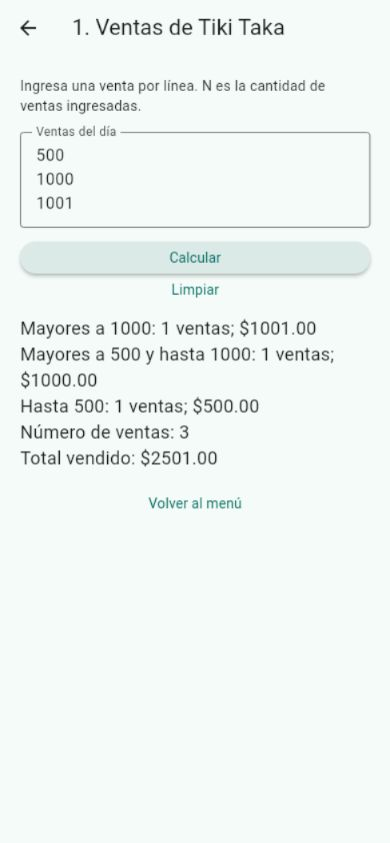
\includegraphics[height=6cm]{evidencias/ventas_web.jpg}}{}
\caption{Menú ejecutado en Android y clasificación de ventas comprobada en el navegador}
\label{fig:ejecucion}
\end{figure}
\clearpage

\subsection{Evidencias de los ejercicios 2 al 5}
\subsection{Evidencia del ejercicio 2}
Los ejercicios se resolvieron mediante ciclos y variables acumuladoras. En el ejercicio 2, un ciclo \texttt{for} inicia el pago en \$10, lo duplica durante los 20 meses y suma cada cuota al total.   

% Captura 1: guarde la primera imagen adjunta como evidencias/ejercicio_2.png.
\evidencia{evidencias/ejercicio_2.png}{Ejecución del ejercicio 2: pagos mensuales duplicados y total acumulado}{fig:ejercicio2}
\subsection{Evidencia del ejercicio 3}
En el ejercicio 3, ciclos anidados recorren las ciudades, tiendas y empleados; cada venta se acumula para obtener los totales de cada tienda, ciudad y de toda la cadena.

% Captura 2: guarde la segunda imagen adjunta como evidencias/ejercicio_3.png.
\evidencia{evidencias/ejercicio_3.png}{Ejercicio 3: cantidades y primeras ventas individuales visibles para C=3, T=4 y N=5}{fig:ejercicio3}

% La captura enviada del ejercicio 3 se corta antes de mostrar todos los subtotales. Tome otra captura desplazándose hasta el resumen final y guárdela con este nombre.
\evidencia{evidencias/ejercicio_3_resumen.png}{Ejercicio 3: ventas totales por tienda, ciudad y cadena}{fig:ejercicio3resumen}


\subsection{Evidencia del ejercicio 4}
En el ejercicio 4, se calcula el sueldo bruto semanal multiplicando las horas trabajadas por el pago por hora y se resta el descuento correspondiente al rango salarial.
% Captura 3: guarde la tercera imagen adjunta como evidencias/ejercicio_4.png.
\evidencia{evidencias/ejercicio_4.png}{Ejecución del ejercicio 4: sueldo bruto, descuento aplicado y sueldo neto de cada trabajador}{fig:ejercicio4}


\subsection{Evidencia del ejercicio 5}
En el ejercicio 5, el capital se actualiza año a año con interés compuesto del 15\%, mediante la expresión $P_{a+1}=P_a(1+0.15)$. Las capturas muestran las pantallas y los resultados de estos cálculos.
% Captura 4: guarde la cuarta imagen adjunta como evidencias/ejercicio_5.png.
\evidencia{evidencias/ejercicio_5.png}{Ejecución del ejercicio 5: capital acumulado al año 2026}{fig:ejercicio5}


\section{Conclusiones}
\begin{enumerate}
\item Se integraron los cinco ejercicios en una aplicación con menú y pantallas independientes.
\item Los ciclos permitieron clasificar ventas, acumular pagos y sumar registros por ciudad, tienda y empleado.
\item Las pruebas confirmaron los resultados seleccionados y el retorno al menú; la ejecución en Android confirmó la apertura de la aplicación.
\end{enumerate}
\section{Recomendaciones}
\begin{enumerate}
\item Respetar el formato de un registro por línea y el orden de las ventas por empleado.
\item Confirmar con la docente los límites del descuento salarial que el enunciado no especificó.
\item Entregar el código fuente sin \texttt{build} ni cachés, y repetir las pruebas después de modificarlo.
\end{enumerate}

\section{Representación del ejercicio 1}
Se utilizó un ciclo \textbf{para}, porque se conoció la cantidad N de ventas. C1, C2 y C3 representaron cantidades; M1, M2 y M3 representaron montos. Los diagramas mostraron el cálculo con entradas válidas. En la app se obtuvo N de la lista y se recorrió cada venta.
\begin{singlespace}
\noindent\begin{minipage}[t]{.43\linewidth}
\textbf{Pseudocódigo}
\begin{lstlisting}
Leer N
C1,C2,C3 <- 0
M1,M2,M3 <- 0
Para i <- 1 hasta N
  Leer venta
  Si venta > 1000
    C1 <- C1 + 1
    M1 <- M1 + venta
  Sino
    Si venta > 500
      C2 <- C2 + 1
      M2 <- M2 + venta
    Sino
      C3 <- C3 + 1
      M3 <- M3 + venta
    FinSi
  FinSi
FinPara
Mostrar C1,C2,C3
Mostrar M1,M2,M3
Mostrar M1 + M2 + M3
\end{lstlisting}
\end{minipage}\hfill
\begin{minipage}[t]{.54\linewidth}
\centering\textbf{Diagrama de flujo}\\[4pt]
\begin{tikzpicture}[x=.64cm,y=.64cm,font=\scriptsize,every node/.append style={inner sep=2pt}]
\node[terminal] (ini) at (0,0) {Inicio};
\node[entrada] (leer) at (0,-1.2) {Leer N};
\node[proceso] (init) at (0,-2.5) {C1,C2,C3=0\\M1,M2,M3=0; i=1};
\node[decision] (ciclo) at (0,-4) {$i\leq N$};
\node[entrada] (venta) at (0,-5.5) {Leer venta};
\node[decision] (mil) at (0,-7) {venta $>1000$};
\node[proceso,text width=1.5cm] (g1) at (-2.8,-8.7) {C1=C1+1\\M1=M1+venta};
\node[decision] (quin) at (2.1,-8.7) {venta $>500$};
\node[proceso,text width=1.5cm] (g2) at (.2,-10.5) {C2=C2+1\\M2=M2+venta};
\node[proceso,text width=1.5cm] (g3) at (3.2,-10.5) {C3=C3+1\\M3=M3+venta};
\node[proceso,text width=1.2cm] (inc) at (0,-12.1) {i=i+1};
\node[entrada,text width=1.5cm] (sal) at (-3.3,-5.6) {Mostrar C1--C3, M1--M3 y total};
\node[terminal] (fin) at (-3.3,-7.1) {Fin};
\draw[flecha] (ini)--(leer);\draw[flecha] (leer)--(init);\draw[flecha] (init)--(ciclo);
\draw[flecha] (ciclo)--node[right]{Sí}(venta);\draw[flecha] (venta)--(mil);
\draw[flecha] (ciclo.west)-|node[above,pos=.35]{No}(sal.north);
\draw[flecha] (sal)--(fin);
\draw[flecha] (mil.west)-|node[above,pos=.3]{Sí}(g1.north);
\draw[flecha] (mil.east)-|node[above,pos=.3]{No}(quin.north);
\draw[flecha] (quin.west)-|node[above,pos=.3]{Sí}(g2.north);
\draw[flecha] (quin.east)-|node[above,pos=.3]{No}(g3.north);
\draw[flecha] (g1.south)|-(inc.west);
\draw[flecha] (g2.south)--(g2.south |- inc.north)--(inc.north);
\draw[flecha] (g3.south)|-(inc.east);
\draw[flecha] (inc.south)--(0,-13)--(5,-13)--(5,-4)--(ciclo.east);
\end{tikzpicture}
\end{minipage}
\par\vspace{8pt}
\noindent\textbf{Diagrama N/S}
\begin{center}
\begin{tikzpicture}[x=1cm,y=.55cm,font=\small]
\draw (0,0) rectangle (14,7);
\draw (0,6.2)--(14,6.2);\node at (7,6.6) {Leer N; C1=C2=C3=0; M1=M2=M3=0};
\draw (.6,1)--(.6,6.2);\node[rotate=90] at (.3,3.6) {Para i = 1 hasta N};
\draw (.6,5.4)--(14,5.4);\node at (7.3,5.8) {Leer venta};
\draw (.6,5.4)--(5,4.4)--(14,5.4);\draw (.6,4.4)--(14,4.4);
\node at (7.3,5.08) {¿venta $>1000$?};\node at (1.4,4.65) {Sí};\node at (13.2,4.65) {No};
\draw (5,1)--(5,4.4);\node[align=center] at (2.8,2.7) {C1=C1+1\\M1=M1+venta};
\draw (5,4.4)--(9.5,3.4)--(14,4.4);\draw (5,3.4)--(14,3.4);
\node at (9.5,4.1) {¿venta $>500$?};\node at (5.6,3.65) {Sí};\node at (13.4,3.65) {No};
\draw (9.5,1)--(9.5,3.4);
\node[align=center] at (7.25,2.2) {C2=C2+1\\M2=M2+venta};
\node[align=center] at (11.75,2.2) {C3=C3+1\\M3=M3+venta};
\draw (0,1)--(14,1);\node at (7,.5) {Mostrar cantidades, montos y total M1+M2+M3};
\end{tikzpicture}
\end{center}
\end{singlespace}

\clearpage
\section{Representación del ejercicio 2}
Se utilizó un ciclo \textbf{para} con 20 repeticiones. En cada mes se mostró el pago, se sumó al total y se duplicó para la siguiente iteración. El pago mensual siguió $p_m=10\cdot2^{m-1}$.
\begin{singlespace}
\noindent\begin{minipage}[t]{.43\linewidth}
\textbf{Pseudocódigo}
\begin{lstlisting}
pago <- 10
total <- 0
Para mes <- 1 hasta 20
  Mostrar mes, pago
  total <- total + pago
  pago <- pago * 2
FinPara
Mostrar total
\end{lstlisting}
\end{minipage}\hfill
\begin{minipage}[t]{.54\linewidth}
\centering\textbf{Diagrama de flujo}\\[4pt]
\begin{tikzpicture}[
  font=\footnotesize,
  e2terminal/.style={draw,rounded corners,minimum width=1.4cm,
    minimum height=.5cm,align=center,inner sep=3pt},
  e2proceso/.style={draw,rectangle,text width=2.9cm,
    minimum height=.65cm,align=center,inner sep=4pt},
  e2decision/.style={draw,diamond,aspect=2,text width=1.5cm,
    align=center,inner sep=2pt},
  e2entrada/.style={draw,trapezium,trapezium left angle=75,
    trapezium right angle=105,text width=2cm,
    align=center,inner sep=4pt},
  e2flecha/.style={-{Stealth[length=2mm]}}
]
\node[e2terminal] (ini) {Inicio};
\node[e2proceso,below=4mm of ini] (init)
  {$pago\gets10$\\$total\gets0$\\$mes\gets1$};
\node[e2decision,below=5mm of init] (ciclo) {$mes\leq20$};
\node[e2entrada,below=6mm of ciclo] (mostrar)
  {Mostrar\\mes y pago};
\node[e2proceso,below=4mm of mostrar] (sum)
  {$total\gets total+pago$};
\node[e2proceso,below=4mm of sum] (dup)
  {$pago\gets pago\cdot2$\\$mes\gets mes+1$};
\node[e2entrada,text width=1.3cm,right=8mm of ciclo,yshift=-1.5cm]
  (sal) {Mostrar\\total};
\node[e2terminal,below=4mm of sal] (fin) {Fin};
\draw[e2flecha] (ini.south)--(init.north);
\draw[e2flecha] (init.south)--(ciclo.north);
\draw[e2flecha] (ciclo.south)--node[right]{Sí}(mostrar.north);
\draw[e2flecha] (mostrar.south)--(sum.north);
\draw[e2flecha] (sum.south)--(dup.north);
\draw[e2flecha] (ciclo.east)-|node[above,pos=.25]{No}(sal.north);
\draw[e2flecha] (sal.south)--(fin.north);
\draw[e2flecha] (dup.south)--++(0,-4mm)--++(-2.4cm,0)
  |- (ciclo.west);
\end{tikzpicture}
\end{minipage}
\par\vspace{1cm}
\noindent\textbf{Diagrama N/S}
\begin{center}
\begin{tikzpicture}[x=1cm,y=1cm,font=\small]
% Cabecera horizontal del ciclo para evitar texto vertical superpuesto.
\draw (0,0) rectangle (12,4.7);
\draw (0,3.8)--(12,3.8);
\node at (6,4.25) {$pago\gets10$; $total\gets0$};
\node at (6,3.5) {Para $mes=1$ hasta $20$};
\draw (.45,3.2)--(12,3.2);
\draw (.45,.8)--(.45,3.2);
\draw (.45,2.4)--(12,2.4);
\draw (.45,1.6)--(12,1.6);
\node at (6.225,2.8) {Mostrar mes y pago};
\node at (6.225,2) {$total\gets total+pago$};
\node at (6.225,1.2) {$pago\gets pago\cdot2$};
\draw (0,.8)--(12,.8);
\node at (6,.4) {Mostrar total};
\end{tikzpicture}
\end{center}
\end{singlespace}


\clearpage
\begin{thebibliography}{5}
\bibitem[Android Developers(2026)]{android}
Android Developers. (2026, 22 de septiembre). \textit{Introduction to activities}. \url{https://developer.android.com/guide/components/activities/intro-activities}
\bibitem[Dart(2025)]{dart}
Dart. (2025, 5 de mayo). \textit{Loops}. \url{https://dart.dev/language/loops}
\bibitem[Flutter(2026a)]{navegacion}
Flutter. (2026a, 29 de septiembre). \textit{Navigate to a new screen and back}. \url{https://docs.flutter.dev/cookbook/navigation/navigation-basics}
\bibitem[Flutter(2026b)]{rutas}
Flutter. (2026b, 29 de septiembre). \textit{Navigate with named routes}. \url{https://docs.flutter.dev/cookbook/navigation/named-routes}
\bibitem[Nassi y Shneiderman(1973)]{ns}
Nassi, I., \& Shneiderman, B. (1973). Flowchart techniques for structured programming. \textit{ACM SIGPLAN Notices, 8}(8), 12--26. \url{https://www.cs.umd.edu/users/ben/papers/Nassi1973Flowchart.pdf}
\end{thebibliography}
\end{document}


